\chapter{Advanced Encryption standard}\label{ch:AES}
The AES is based on an SP-network and is fast both in hardware as well as 
software. Rijndael, which is used in AES, has key-sizes of at least 128 bits, 
block lengths of 128 bits, 8 to 8 bit S-boxes and a minimum of 10 rounds of 
repetition \citep[p. 79]{Stinson:2006}. It is a symmetric-key algorithm with a 
fixed block size of 128 bits, where the key-size can vary between 128, 192 or 
256 bits. The number of cycles needed to convert the plaintext into ciphertext 
depends on the size of the key. The 128-bit key requires 10 cycles of 
repetitions (rounds). The 192-bit key requires 12 rounds and the 256-bit key 
requires 14 rounds \citep[p. 103]{Stinson:2006}.

\section{Method}
The AES consists of a number of steps that are repeated for each block to be 
encoded. The steps to be performed are, according to \citet{Stinson:2006}:

\emph{Set-up steps}
\begin{enumerate}
\item KeyExpansion - Produce round keys.
\item InitialRound - Combine each byte of the state with a byte of round key.
\end{enumerate}
\emph{Steps performed in rounds}
\begin{enumerate}
\item SubBytes - Each byte is \emph{substituted} using the Rijndael's S-box.
\item ShiftRows - The rows of the state matrix are \emph{permutated}.
\item MixColums - The columns of the matrix are multiplicated with a matrix.
\item AddRoundKey - The state matrix is once again combined with round-keys.
\end{enumerate}
\emph{In the final round we do everything except the MixColumns step}
\begin{enumerate}
\item SubBytes
\item ShiftRows
\item AddRoundKey
\end{enumerate}

The ciphertext is then defined as the state-matrix \citep[p. 103]{Stinson:2006}. 
As mentioned in section \ref{ch:ConfDiff} (\nameref{ch:ConfDiff}), both 
confusion and diffusion are nescessary. They can be seen in the SubBytes and 
ShiftRows steps above. These steps also performs whitening, which strengthens the cipher. Whitening is, as mentioned in \ref{ch:ConfDiff}, performed through an 
XOR between the subkey and the data.

The KeySchedule is explained in section \ref{sec:KeySch}.

\subsection{InitialRound}
This is simply an initial AddRoundKey.

\subsection{SubBytes}
In the SubBytes step, each byte is sent to a Rijndael S-box (which is basically
 a lookup table) where they are substituted in a non-linear fashion. This gives 
us a substituted state matrix.

\subsection{ShiftRows}
The next step is called the ShiftRows step, which left-shift the rows n-1 
steps where n is the index of the row. This means that the first row is left 
as it is, the second row is shifted one step, the third row is shifted two 
steps, and the fourth row is shifted three steps.

\subsection{MixColumns}
In the MixColumns step, the four bytes of each row are combined through a matrix 
multiplication. The MixColumns function takes four bytes as input and multiplies 
them with a fixed matrix (figure \ref{matrix:rijMix} in appendix 
\ref{app:misc}). While this might seem simple, it really is not. The 
multiplication makes sure that each input byte affect all output bytes.
\citep{Angelfire}

The matrix is multiplicated from the left to the vector (4x4 * 4x1 = 4x1) which 
is a column from the state-matrix. Multiplication with 1 means that the value 
is left untouched. Multiplication by 2 means left shift, then XOR with 0x1B is 
the value is larger than 0xFF. Multiplication with 3 means left-shift (including 
XOR with 0x1B if the value exceeds 0xFF), then XOR with the initial value. 
Addition is replaced with XOR, due to the calculations taking place in 
GF(\(2^8\)) \Warning[DOODOO]{Add a reference to Galois fields}.

%Next a subkey is derived from the main key using Rijndael’s key schedule. The 
%subkey is the same size as the state matrix. Each element in the state matrix 
%is then combined to the corresponding element in the subkey using a bitwise XOR.

\subsection{AddRoundKey}
Each of the 16 bytes of the state is combined with a byte of the round key 
using bitwise xor. They are then combined to a state matrix (figure 
\ref{matrix:state} in appendix \ref{app:misc}) containing 4x4 bytes.

\section{KeyExpansion}\label{sec:KeySch}
To generate round keys from the cipher key, we use the Rijndael's key schedule. 
This is done since AES requires a separate 128-bit round key for each round, 
plus one extra key for the initialization which means that the AES-128 requires 
176 bytes, since AES-128 consists of 10 rounds. 

%Beskrivningen här behöver antingen vara en punktlista, som jag skulle kunna försöka hitta via referenser och dylikt. Eller en flowchart. Men isåfall måste jag kunna berätta varifrån jag har fått faktan till hur jag producerat min flowchart.

The schedule consists of a loop, and a key-schedule core. The schedule core is 
the part that branches out from the check if c modulo 16 is zero. The entire 
KeyExpansion can be viewed in Figure \ref{img:keysch}. To change the key schedule
to fit a key size of 192 bits, you simply change the value c is compared to in 
the first branch in the flowchart from 176 to 206. 

\begin{figure}
  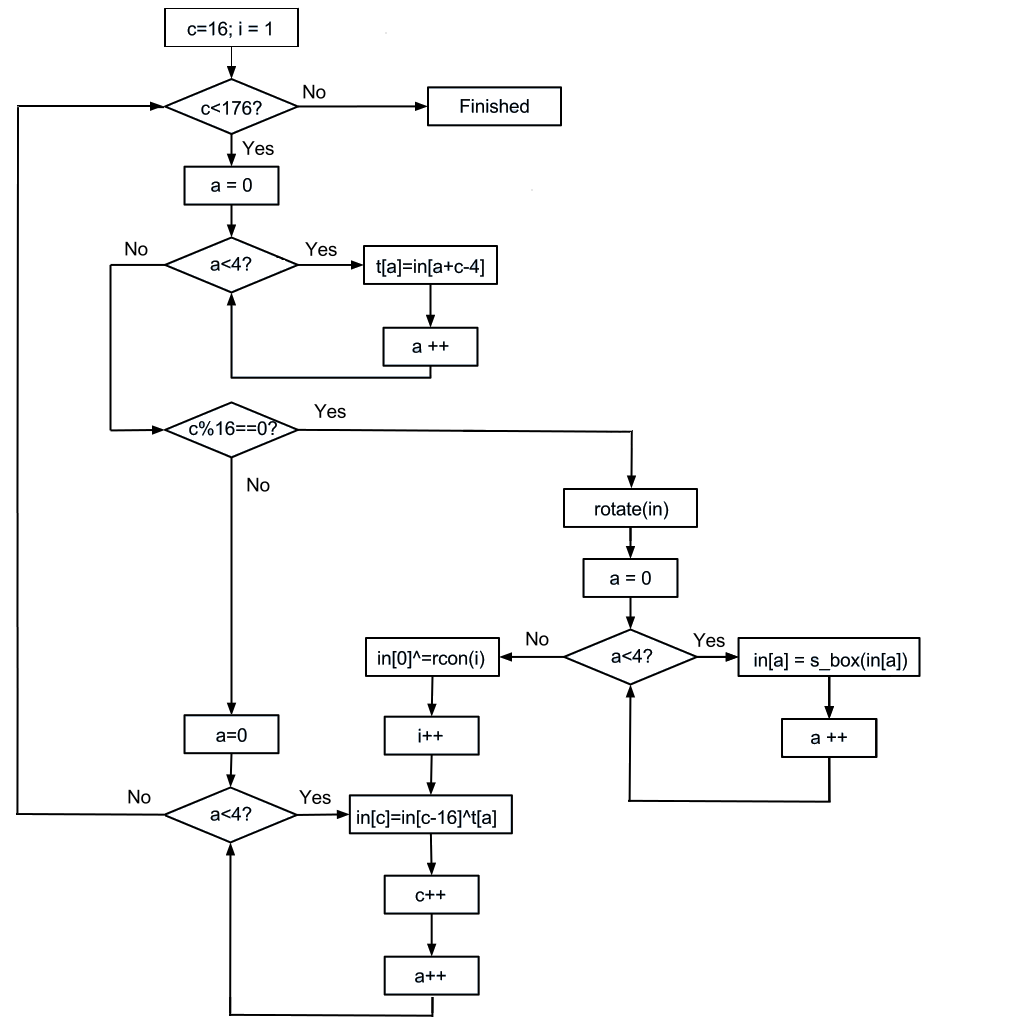
\includegraphics[width=\textwidth]{keyschedule}
  \caption{Flowchart of the key schedule}
  \label{img:keysch}
\end{figure}

\subsection{Key-schedule core}\label{sec:kCore}
The key-schedule core takes an input of 4 bytes (32 bits) which it then rotates 
1 byte (8 bits) to the left. Let us say that our key is \emph{AB CD EF 01}. This 
would give us the key \emph{CD EF 01 AB} after the rotation. This operation is 
also called the RotWord-operation \citep[p. 107]{Stinson:2006}. The next step is 
to apply Rijndael's S-box to each of these bytes, giving us 4 new bytes. The 
bytes {AB CD EF 01} would give us {62 BD DF 7C} when input in the Rijndael 
S-box (Figure \ref{matrix:rijSbox}).

The left-most byte is then XORed with a value from the Rcon function depending 
on what round you are currently at. You can read more about the Rcon function in 
section \ref{ch:Rcon}.

\subsection{Rijndael's S-Box}
Rijndael's S-box takes an input byte which it transforms according to a matrix 
(figure \ref{matrix:rijSbox} in appendix \ref{app:misc}). Where the most 
significant nibble is placed on the Y axis, and the least significant nibble 
is set on the X axis. Let us say we have an input of 0x31, then 0xC7 would be 
output from the Rijndael's S-box.

 \subsection{Rcon} \label{ch:Rcon}
The value input into the Rcon function depends on what round you are currently 
at. Which means that you would choose Rcon(1) for the first round, Rcon(2) for 
the second round, and so on. The values in the Rcon array are calculated 
mathematically, but might as well be accessed through a simple vector or such.

%I translated the steps to be performed in the Rcon function into a flowchart which can be viewed in figure \ref{app:flowchart} in appendix \ref{app:misc}. 

If the input value is 0 or 1, we just return that value, otherwise the 
following steps are performed \citep{RijndaelKeySchedule}. This can also be 
replaced by an S-box where you input your byte, and get another back, since the 
input byte is just used as a counter that decides how many times you perform 
steps \ref{item:step1} through \ref{item:step3} 
\Warning[TODO]{You need more reliable sources than WIKIPEDIA!}.

\begin{enumerate}
\item Set a variable c to 0x01.
\item If the input-value does not equal 1, set variable b to c \& 0x80. 
Otherwise, go to \ref{item:exit_loop}. 
\label{item:step1}
\item Left shift c one step.
\item If b is equal to 0x80 proceed to \ref{item:step2}, otherwise go to 
\ref{item:step3}.
\item Store the result of a bitwise XOR between c and 0x1B in c.
\label{item:step2}
\item The input value is decreased by one, and we go back to \ref{item:step1}.
\label{item:step3}
\item We set the output to c.
\label{item:exit_loop}
\end{enumerate}
